\documentclass[english]{article}
\usepackage[english]{babel} 
\usepackage[T1]{fontenc}
\usepackage[utf8x]{inputenc}
\usepackage{float}
\usepackage{graphicx}

\makeatletter
\usepackage[a4paper,top=2cm,bottom=2cm,left=2cm,right=2cm]{geometry}
\usepackage{enumitem}
\usepackage{subfig}
\usepackage{amsthm}
\usepackage{amsmath}
\usepackage{epstopdf}
\usepackage{fancyhdr}
\usepackage{booktabs,array}
\usepackage{hyperref}

\hyphenation{english}
\makeatother

\usepackage{babel}


\usepackage{listings}
\usepackage{xcolor} % for setting colors

% set the default code style
\lstset{
    frame=tb, % draw a frame at the top and bottom of the code block
    tabsize=4, % tab space width
    showstringspaces=false, % don't mark spaces in strings
    numbers=left, % display line numbers on the left
    commentstyle=\color{gray}, % comment color
    keywordstyle=\color{blue}, % keyword color
    stringstyle=\color{red} % string color
}


\begin{document}
\begin{titlepage}

	\begin{center}
		\begin{Large} \textbf{UNIVERSITY OF PADOVA} \\
		\end{Large} \vspace{1cm}
		\vspace{3cm}
		\begin{Large} Embedded Real--Time Control \end{Large}
		\par\end{center}

	\begin{center}
		\begin{Large}Laboratory report\\
		\end{Large}
		\par\end{center}

	\begin{center}
		\vspace{2cm}
		\begin{figure}[!htb]
			\centering 
\includegraphics[width=8cm]{figures/unipd-logo.png}\\

		\end{figure}

		\par\end{center}

	\begin{center}
		\vspace{2cm}
		\begin{Large} Names - (Student ID Numbers)  \\
		\end{Large} \vspace{2cm}
		\begin{Large} Academic Year 2021-2022 \end{Large}
		\par\end{center}

\end{titlepage}

\tableofcontents
\newpage

\section{General notes}
	\paragraph{}
	This report was made as part of evaluation of course Embedded Real-Time Control at UNIPD.
	In labs we were using and all development was done on device named TurtleBot (see picture \ref{fig:turtlebot}).
	As software development tool was used STM32 CUBE IDE.

	\paragraph{}
	We are using microcontroller from STM32F7 series, part of STMicroelectronics' STM32 family, is based on the ARM Cortex-M7 core, operating at frequencies up to 216 MHz. 
	It is designed for high-performance embedded applications that require substantial processing power combined with real-time capabilities. 
	The STM32F7 features up to 2 MB of dual-bank Flash memory, up to 512 KB of SRAM (with additional TCM memory), and includes an integrated 
	Floating Point Unit (FPU) and Digital Signal Processing (DSP) instructions for efficient signal processing tasks. Key peripherals include 
	high-speed USB OTG (with support for full-speed and high-speed modes), multiple 12-bit ADCs and DACs, timers with encoder and PWM modes,
	as well as extensive connectivity options such as UART, SPI, I²C, CAN, SDIO, and Ethernet MAC with IEEE 1588 support.
	The series also includes an L1 cache (I-cache and D-cache), Chrom-ART Accelerator for graphical applications, 
	and flexible memory interfaces for external SDRAM, SRAM, or NOR/NAND Flash.
	These features make the STM32F7 well-suited for applications involving advanced user interfaces, audio processing, motor control,
	and industrial automation.

	\begin{figure}[H]
		\centering
		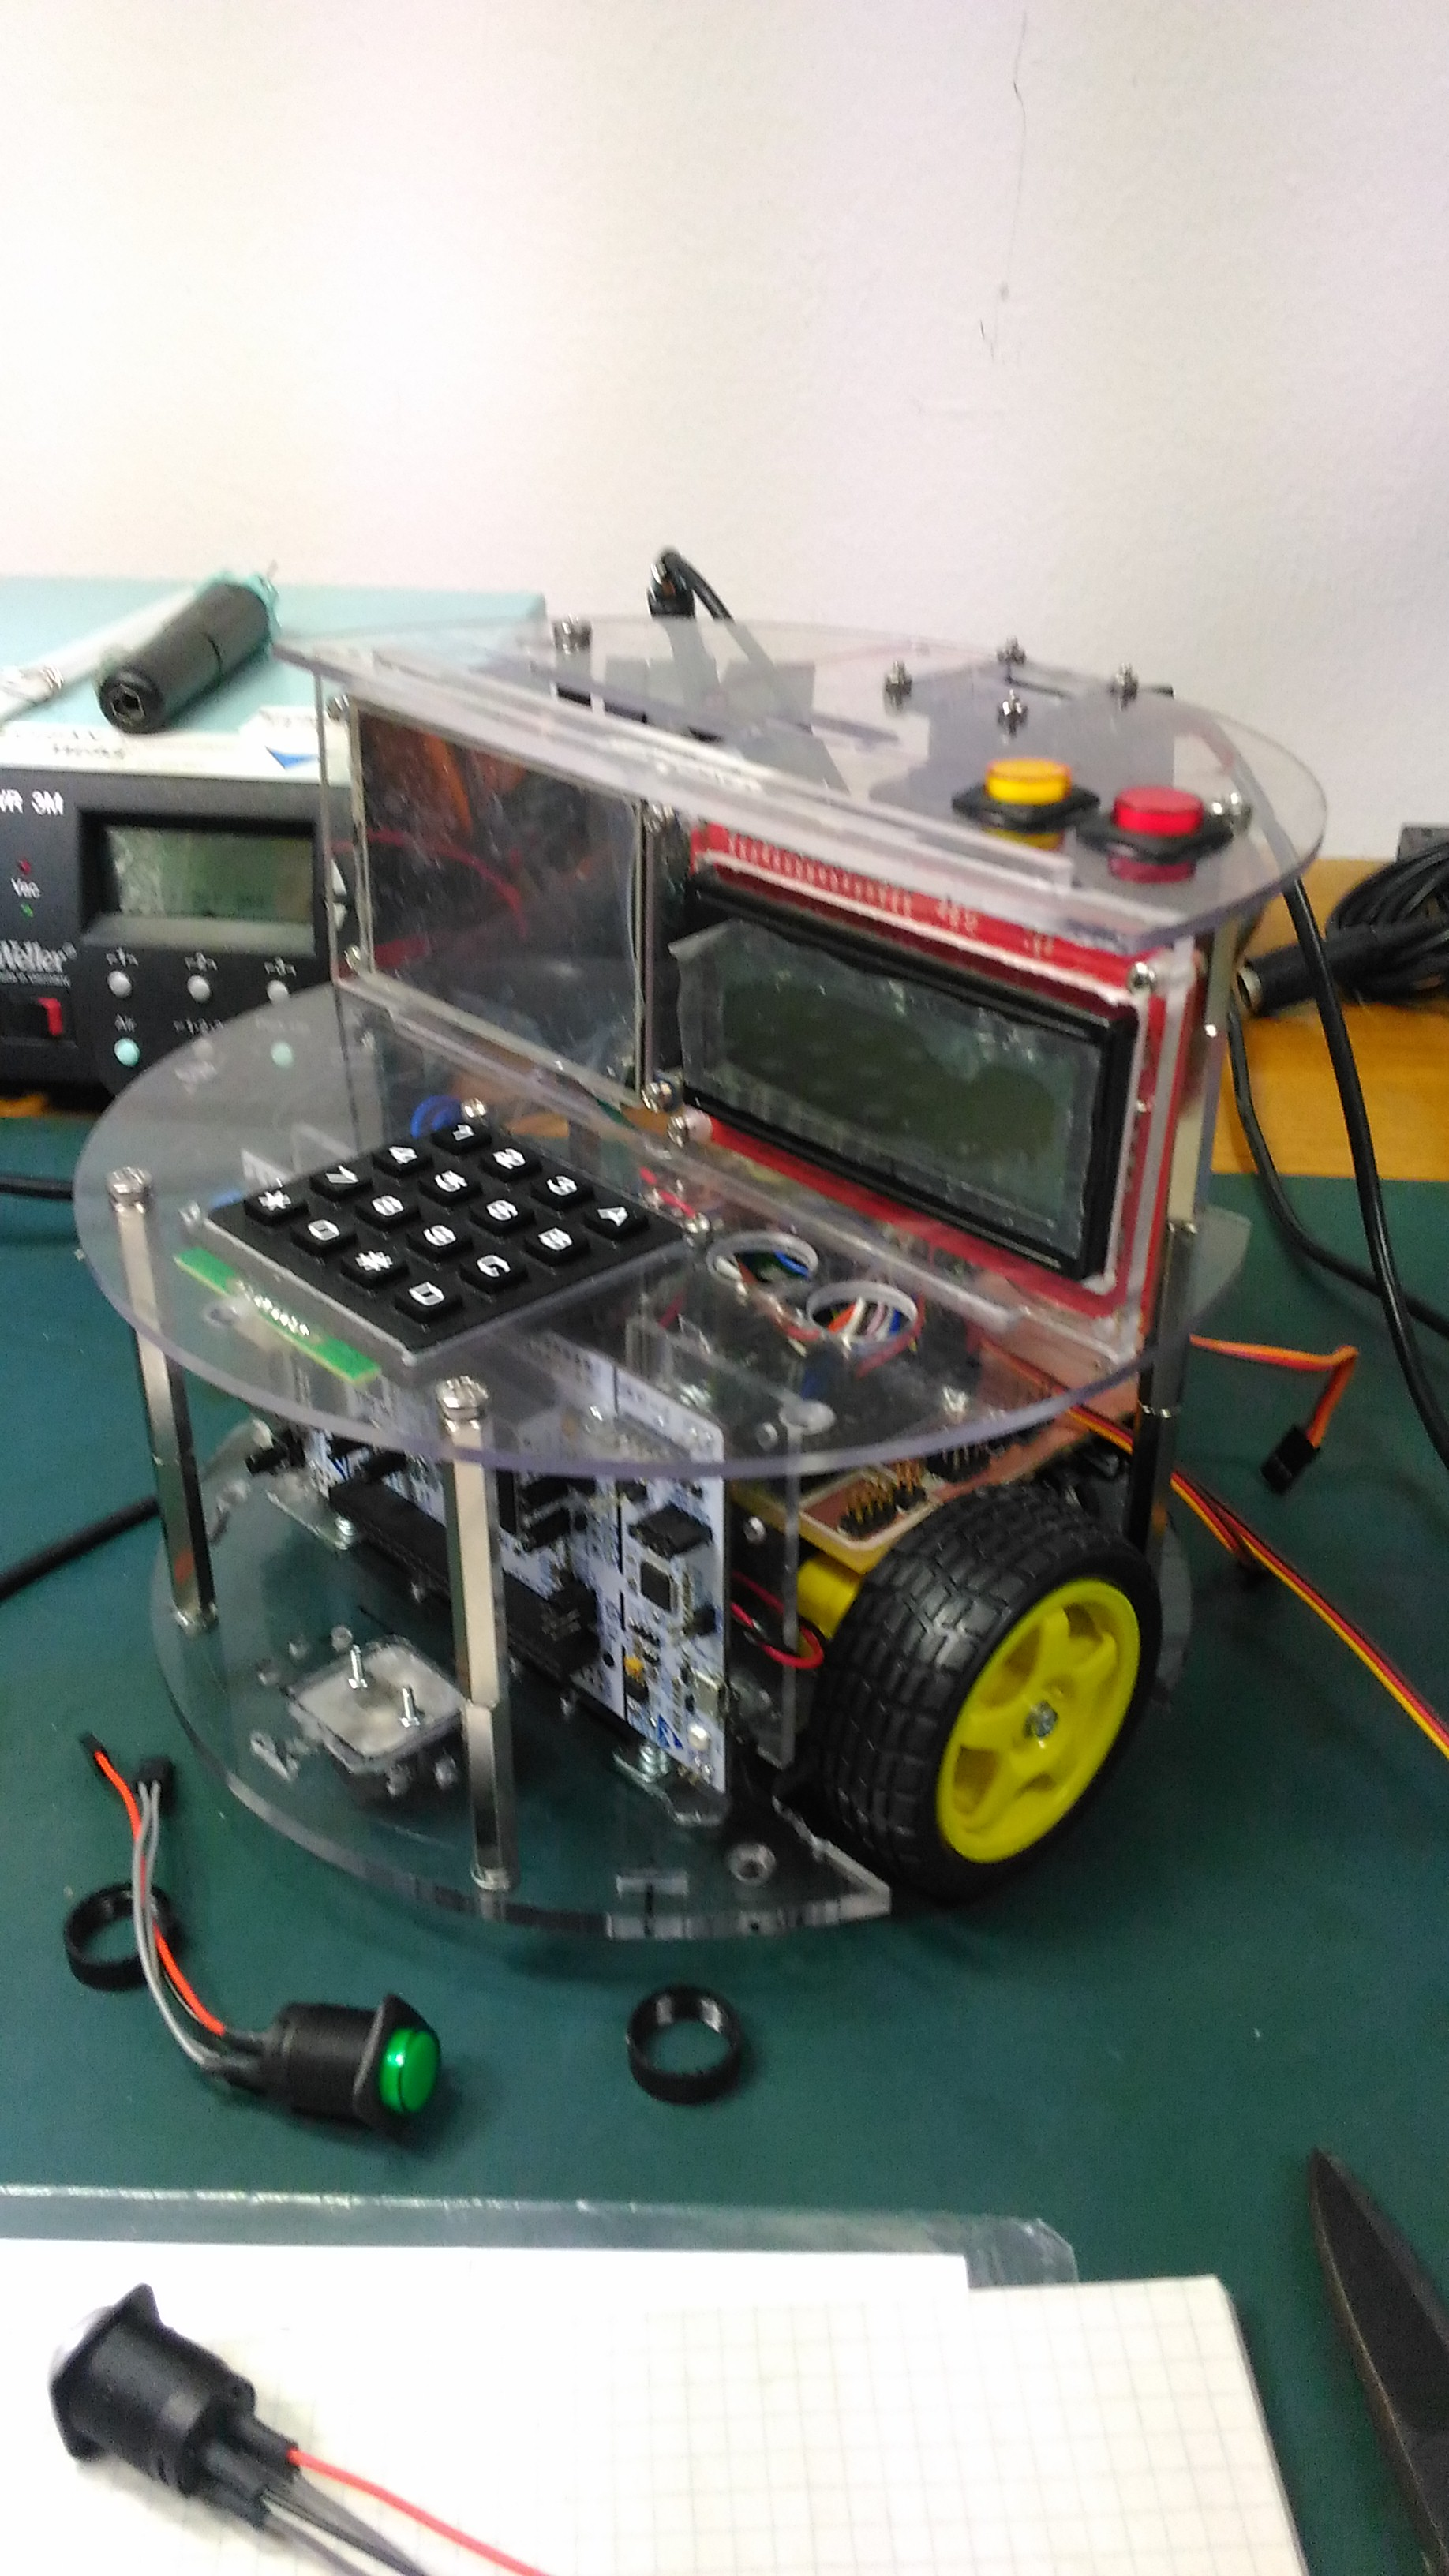
\includegraphics[width=0.5\textwidth]{figures/turtlebot_1.jpg}
		\caption{The TurtleBot}
		\label{fig:turtlebot}
	\end{figure}

	\begin{figure}[H]
		\centering
		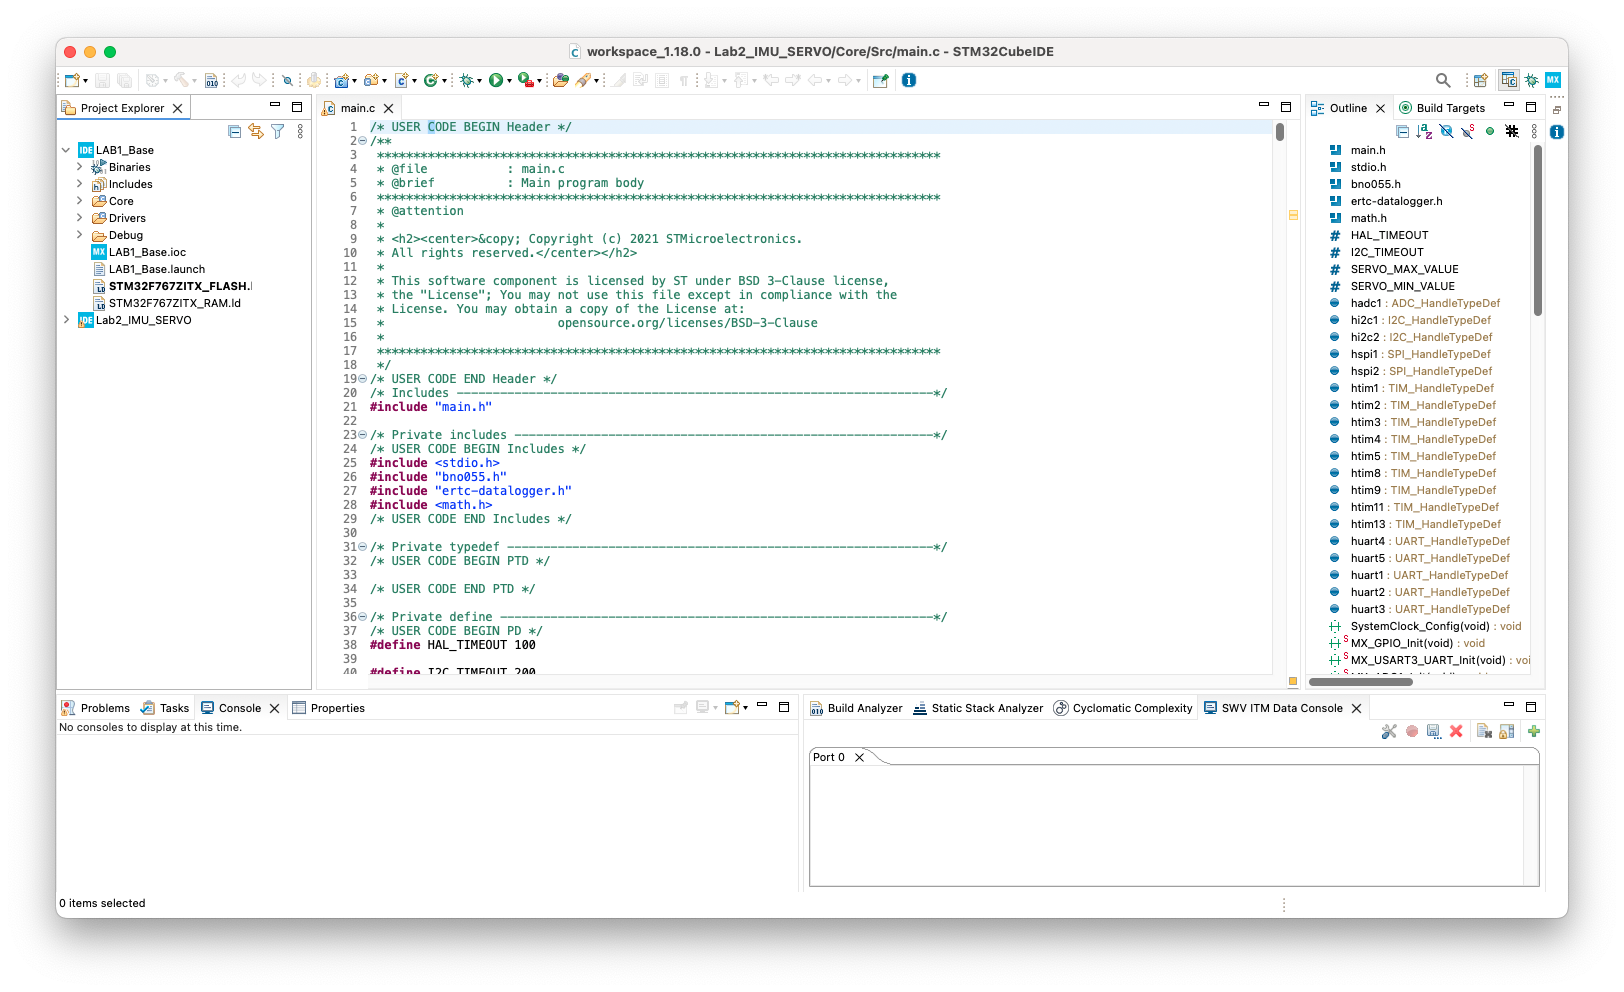
\includegraphics[width=1\textwidth]{figures/cube_ide.png}
		\caption{example from STM32 cube IDE}
		\label{fig:cube}
	\end{figure}
\section{Laboratory 1} %todo: add screenshot from console.

	\paragraph{}
	Target of the first lab was to establish I2C communication between mcu STM32 and I/O expander SX1509. And to read
	the data from the keypad and the line sensor with help of this expander. See configuration on picture \ref{fig.lab1.config}.

	\begin{figure}[H]
		\centering
		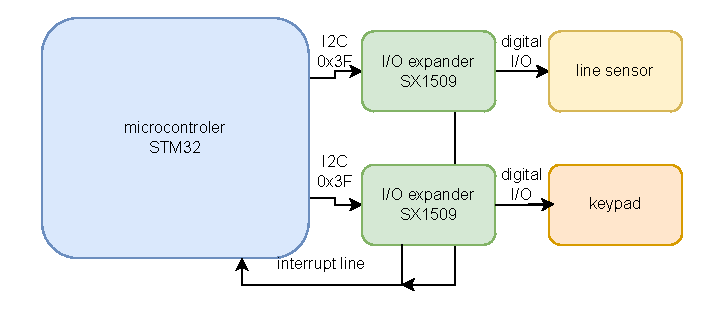
\includegraphics[width=0.8\textwidth]{figures/config_stm_lab1.pdf}
		\caption{The TurtleBot}
		\label{fig.lab1.config}
	\end{figure}

	\subsection{SX1509 I/O expander}

		\paragraph{}
		We are using 16-ch digital I/O expander SX1509 \cite{sx1509}. Device has two I/O banks, represented by two registers in device memory
		of address 0x27 and 0x28. The I2C address of device is configurable by 2 address pins. Up to 4 devices could be at one line. 
		We are using addresses 0x3E and 0x3F since we have 2 devices. Chip has built in debouncing, keypad engine and LED driver. See scheme on the pictre \ref{fig.lab1.sx1509}

		\begin{figure}[H]
			\centering
			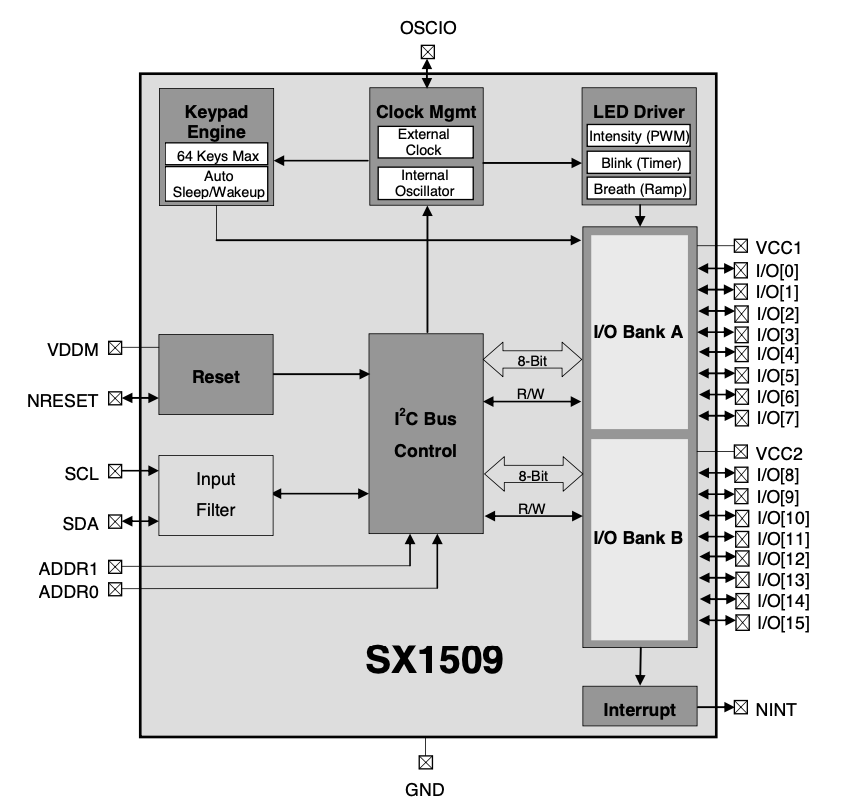
\includegraphics[width=0.6\textwidth]{figures/sx1509.png}
			\caption{SX1509 block scheme}
			\label{fig.lab1.sx1509}
		\end{figure}

	\subsection{Line sensor}

		\paragraph{}
		TurtleBot has Pololu QTR sensor\cite{line_sensor} onboard, version with 8 channels and analog output. Each one of the outputs is connected to one of the
		digital inputs of SX1509. Internal logic of expander converts signal to digital one when is voltage higher/lower than treshold. Order of bits coresponds to physical state of the sensor. Principle of sensor is shown on picture \ref{fig.lab1.line_sensor}.

		\begin{figure}[H]
			\centering
			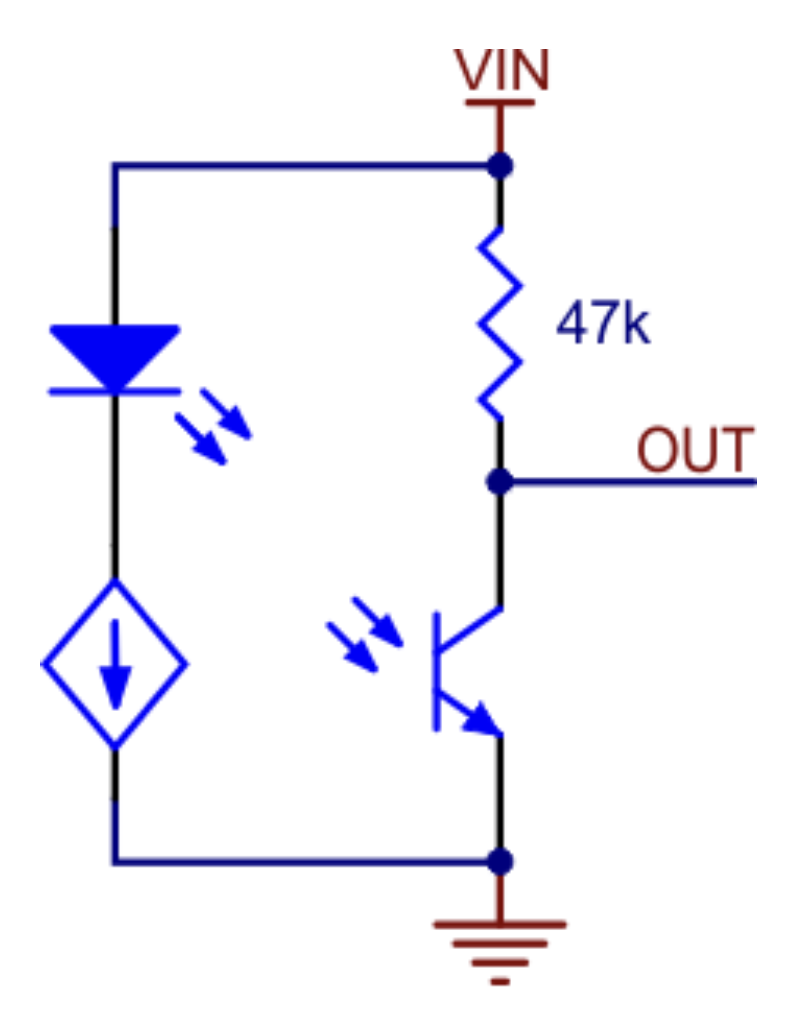
\includegraphics[width=0.3\textwidth]{figures/line_sensor.png}
			\caption{Scheme of single unit from line sensor}
			\label{fig.lab1.line_sensor}
		\end{figure}
		
	\subsection{Keypad}
		\paragraph{}
		Classical 4x4 matrix keypad is used. Digital signal is connected to I/O expander. Rows are connected to the one bank (0x28) and colums (0x27) to the other one,
		so four low bits of represents the keys. See keyboard configuration on picture \ref{fig.lab1.keypad}.

		\begin{figure}[H]
			\centering
			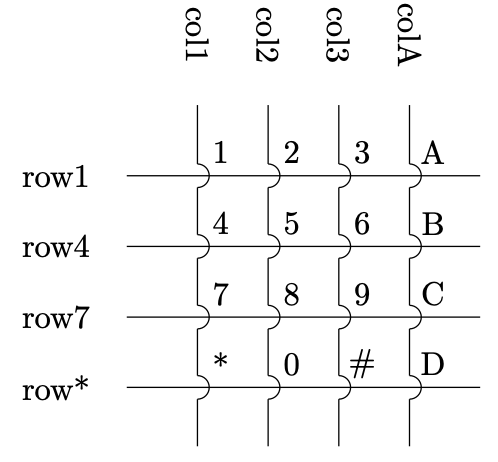
\includegraphics[width=0.4\textwidth]{figures/keypad.png}
			\caption{Scheme of keypad connection}
			\label{fig.lab1.keypad}
		\end{figure}

	\subsection{Laboratory work}
		% \paragraph{main():}
		% In listing \ref{lst.lab1.main} we can see infinite while loop part of main(). We will refer to this later.

		% \begin{lstlisting}[language=C, caption={Keypad callback function}, label={lst.lab1.main} ]
		% 	while (1)
		% 	{
		% 	if(IRQ_GPIO_flag)
		% 	{
		% 		printf("Interrupt on pin: (%d).\n", IRQ_GPIO_pin);

		% 		printf("row register data: %d  ,", GetKeypadPosition(key_rows_data));
		% 		printf("  columns register data: %d",GetKeypadPosition(key_cols_data));
		% 		printf("\n");

		% 		printf("Char pressed: %c", GetCharFromKeypad(GetKeypadPosition(key_rows_data),
		% 		GetKeypadPosition(key_cols_data)));
		% 		printf("\n");

		% 		IRQ_GPIO_flag = 0;
		% 		IRQ_GPIO_pin = 0;
		% 	}

		% 	HAL_Delay(100);
		% 	GetLightSensorStatus(&light_sensor_data);
		% 	printf("line sensor status: %d", light_sensor_data);
		% 	printf("\n");
		% 	}
		% \end{lstlisting}


		\paragraph{Exercise 1 \& Exercise 2:}
		Write an ISR that recognizes and correctly handles the keypad interrupts. You have to properly implement the
		void HAL\_GPIO\_EXTI\_Callback(uint16\_t pin) function. Then print which interrupt has been triggered,i.e.,
		the pin. To be able to receive another interrupt from the keypad, have to read the registers REG\_KEY\_DATA\_1
		and REG\_KEY\_DATA\_2 inside the ISR.

		\paragraph{}
		Extend the code of exercise 1 to handle the keypad interrupt. You have to print which keypad button has been
		pressed.

		\paragraph{}
		We have implemented one callback function, for reading keypad data only when the button is pressed. We are returning
		2 global variables. One for interupt pin number and one as flag, so we can execute appropriate part of code in main.
		Then we calling function to read data from row and colums through I2C. See listing \ref{lst.lab1.callback}.

		\begin{lstlisting}[language=C, caption={Keypad callback function}, label={lst.lab1.callback} ]
	void HAL_GPIO_EXTI_Callback(uint16_t GPIO_Pin)
	{
		IRQ_GPIO_pin = GPIO_Pin;
		IRQ_GPIO_flag = 1;
		HAL_I2C_Mem_Read(&hi2c1, I2C_KEYPAD_ADDRESS, KEYPAD_ROWS_ADDRESS,
		8, key_rows_data, 1, I2C_TIMEOUT);
		HAL_I2C_Mem_Read(&hi2c1, I2C_KEYPAD_ADDRESS, KEYPAD_COLS_ADDRESS,
		8, key_cols_data, 1, I2C_TIMEOUT);
	}
		\end{lstlisting}


		\paragraph{}
		To get character from the keypad, we need to decode the data we received from the expander. For that purpose we have two functions,
		you can see in listing \ref{lst.lab1.keypad}. %In case of second function it would make sense to make it inline, since we only calling 
		%char from array.

		\begin{lstlisting}[language=C, caption={Keypad get cahr functions}, label={lst.lab1.keypad} ]
	uint8_t GetKeypadPosition(uint8_t data)
	{
		if(data == 254)
			return 0;
		else if(data == 253)
			return 1;
		else if(data == 251)
			return 2;
		else
			return 3;
	}


	char GetCharFromKeypad(uint8_t const rows, uint8_t const cols)
	{
		return keypadLayout[rows][cols];
	}
		\end{lstlisting}

		\paragraph{Exercise 3:}
		Write a routine that reads the status of the line sensor and prints it. The routine must check the status with a
        polling period of 100ms.

		\paragraph{}
		We implemented function for reading data form the light sensor (see \ref{lst.lab1.line} ), and we calling this function by polling in main every 
		100 ms. We basically just read device registers trough I2C.

		\begin{lstlisting}[language=C, caption={Keypad get cahr functions}, label={lst.lab1.line} ]
	void GetLightSensorStatus(uint8_t * data)
	{
	HAL_I2C_Mem_Read(&hi2c1, I2C_LIGHT_SENSOR_ADDRESS, LINE_SENSOR_ADDRESS,
	1, data, 1, I2C_TIMEOUT);
	}
		\end{lstlisting}

		\paragraph{Exercise 4:}
		We haven't saved LAB0, since it is not part final evaluation, so we can extend it, but since our LAB0 was working properly, it
		is basically just changing LED delay based on keypad input. That means making a function that returns delay value based on input combination.

	\subsection{Conclusion}
	\paragraph{}
	In this lab we establish I2C communication with two devices and successfully read data from these. We implemented keypad decoder, 
	successfully read data from line sensor and haven't finished exercise 4, because we haven't saved lab0 on flash disk and were not able
	to login to school comuputer for 20 minutes. At least we make theoretical description of the problem, since it is quite trivial. Some
	of the functions are short so it would make sense to make them inline or not using function at all. We are not aiming for the most effective 
	code and we prefer readability. Our code was not compiling with inline versions so we are using regular functions.

\section{Laboratory 2}
\paragraph{}
The aim of this laboratory was to implement an open-loop camera stabilization system on the TurtleBot using data from its IMU and controlling two servo motors to adjust the tilt and the pan of the camera. 

    \subsection{IMU Data Handling}
    \paragraph{}
    The TurtleBot is equipped with a 6-DOF IMU, comprised of a 3-axis accelerometer and 3-axis gyroscope. The accelerometer measures the linear acceleration $ [m/{s}^2] $ along the 3 axes, while the gyroscope measures angular velocity(rad/s) around these axes. The data from the two sensors is available within
    
    \verb|bno055_convert_double_accel_xyz_msq()| and \verb|bno055_convert_double_gyro_xyz_rps()| respectively.  The data provided by the IMU is crucial when estimating the movement and orientation of the robot, particularly for calculating the tilt as follows:

    \begin{equation}
        \theta = sin^{-1}(\frac{a_y}{g})
    \end{equation}
    where $a_y$ is the acceleration along the y axis.

    \subsection{Servo Control}
    \paragraph{}
    The two servo motors controlling the movement are operated via PWM signals generated by TIM6 of the STM32 and the angles are updated with a frequency of 100Hz using the \verb|__HAL_TIM_PeriodElapsedCallback| function and scaled into a safe duty cycle with the \verb|saturate()| function. 
    \begin{lstlisting}[language=C, caption={Angle update function}, label={lst.lab1.line} ]
    TIM_HandleTypeDef * timer6_ptr = &htim6;
    HAL_TIM_PeriodElapsedCallback(timer6_ptr)
    {
    theta = asin(d_accel_xyz.y/G); 
    pan = (int8_t)(-(theta/3.14)*180) + PAN_BIAS;

    angle = angle + ((-(d_gyro_xyz.z*0.1)/3.14)*180.)/10.;

    tilt = (int8_t)angle;
    }
    \end{lstlisting}
    As can be seen in the code, there is a strange phenomenon where dividing the angle update formula by 10 ensures a smooth pan without the need of a filter. While this makes no sense time/frequency-wise (after having done the calculations multiple times), it does in the end provide a very smooth movement.

    \subsection{Data Logging}
    \paragraph{}
    Data logging was performed via the UART interface of the STM32, while using MATLAB to receive and visualize the data in real time with the \verb|serial_datalog()| function. %TODO: introduce matlab graph

    \subsection{Results}
    \textbf{Lab video demonstration:}:\href{https://youtube.com/shorts/imY0JJ4vP6Q?feature=share}{Video Demonstration}
    \paragraph{}
    The camera stabilization performance was captured and logged while the TurtleBot was tilted manually. As seen in the video, the servo effectively counteracts the tilt to maintain camera alignment, without the need of a complementary filter. In the event of a less fortunate camera setup, the complementary filter would have had the following form:
    \begin{equation}
        \theta_{fused} = \alpha \cdot\theta_{gyro} + (1 - \alpha) \theta_{accel}
    \end{equation}
    ,where $\theta_{gyro}$ and $\theta_{accel}$ are two different sensor measurements, from the gyroscope and accelerometer, respectively, thus ensuring a smoother pan.
    

	\section{Laboratory 3}
	\subsection{Design process}
		\paragraph{}
		We implemented motor controler pretty quickly and tested it out. Everything seems working
		just fine, then we decided make final adjustments of the design. Somehow we changed
		few things and computed error with wrong sign. This mistake take big amount of our time, because
		we assumed that implementation is correct and it was working in some way anyway, but just 
		sometimes which is worst kind of mistakes. We implemented jaw controler, but we were having
		problems to tune it and then we found out the problem. Unfortunetly we didnt have enougt time 
		in labs to tune the PID properly.
	\section{Laboratory 4}

% \begin{figure}[!ht]
% 	\centering
% 	\subfloat[The TurtleBot 1 ]
% 	{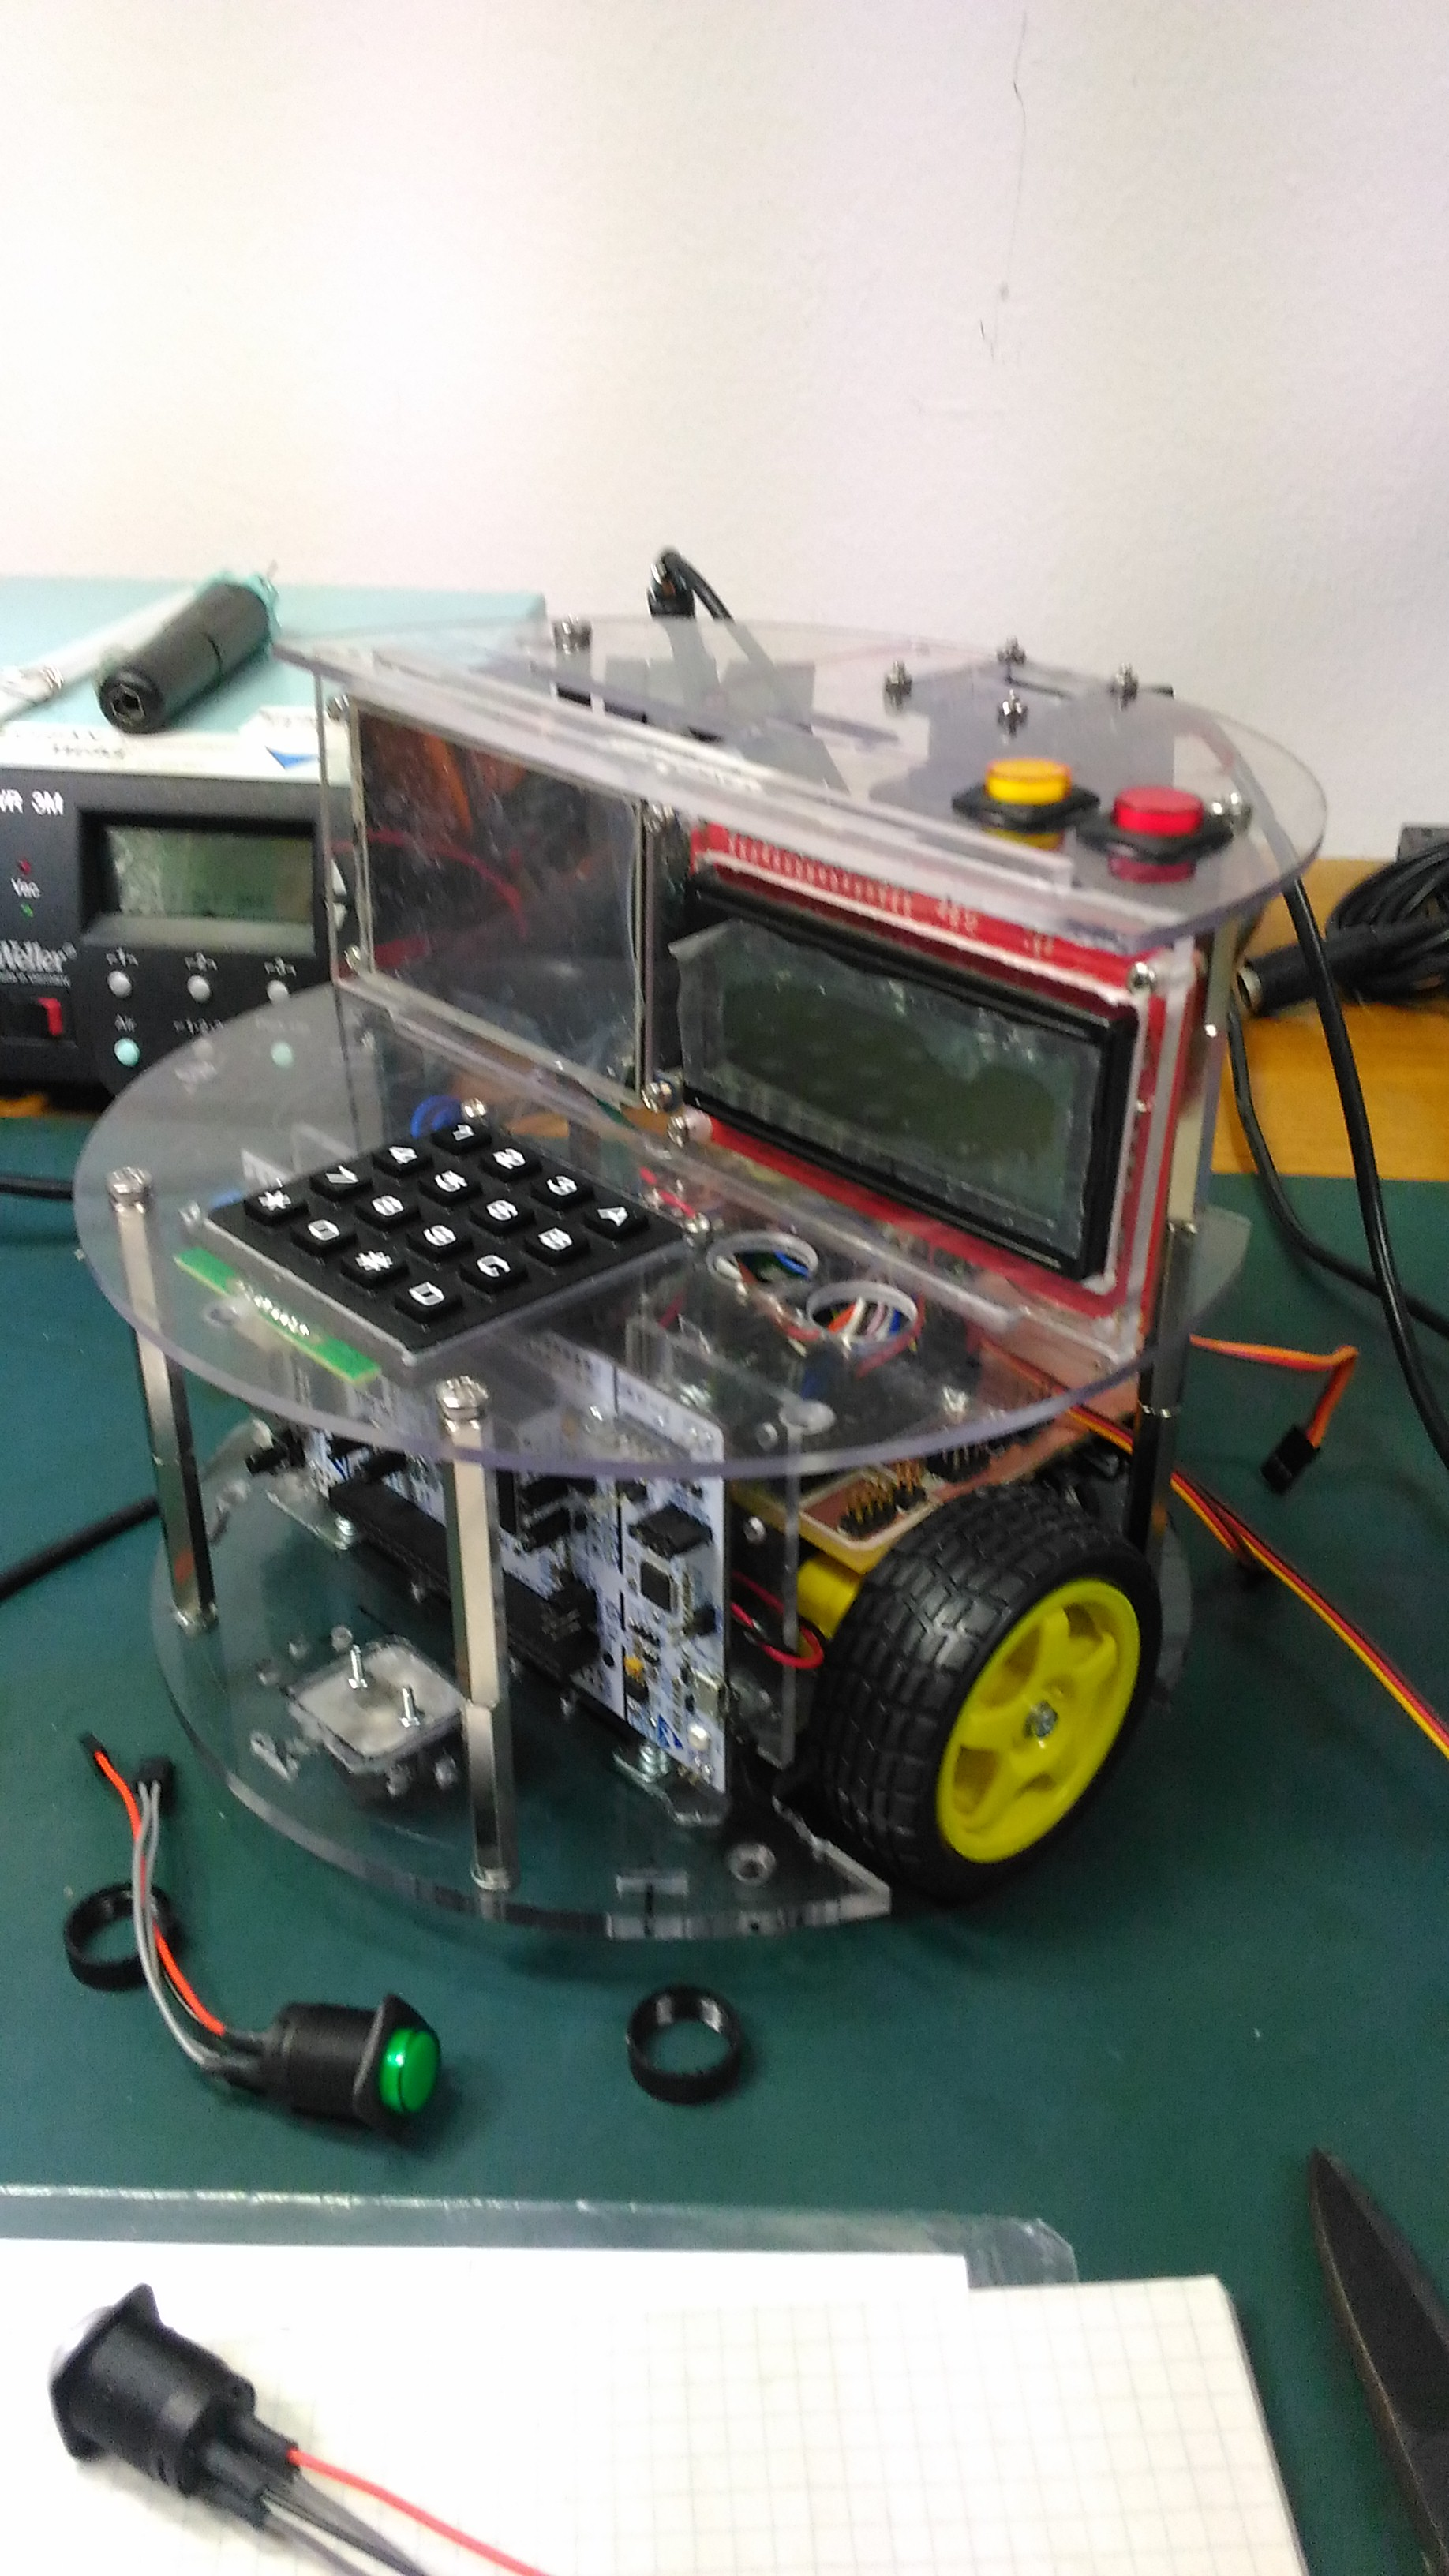
\includegraphics[width=0.3\textwidth,height=0.45\textwidth]{figures/turtlebot_1.jpg}
% 		\label{fig:tbot1}}
% 	\subfloat[The TurtleBot 2]
% 	{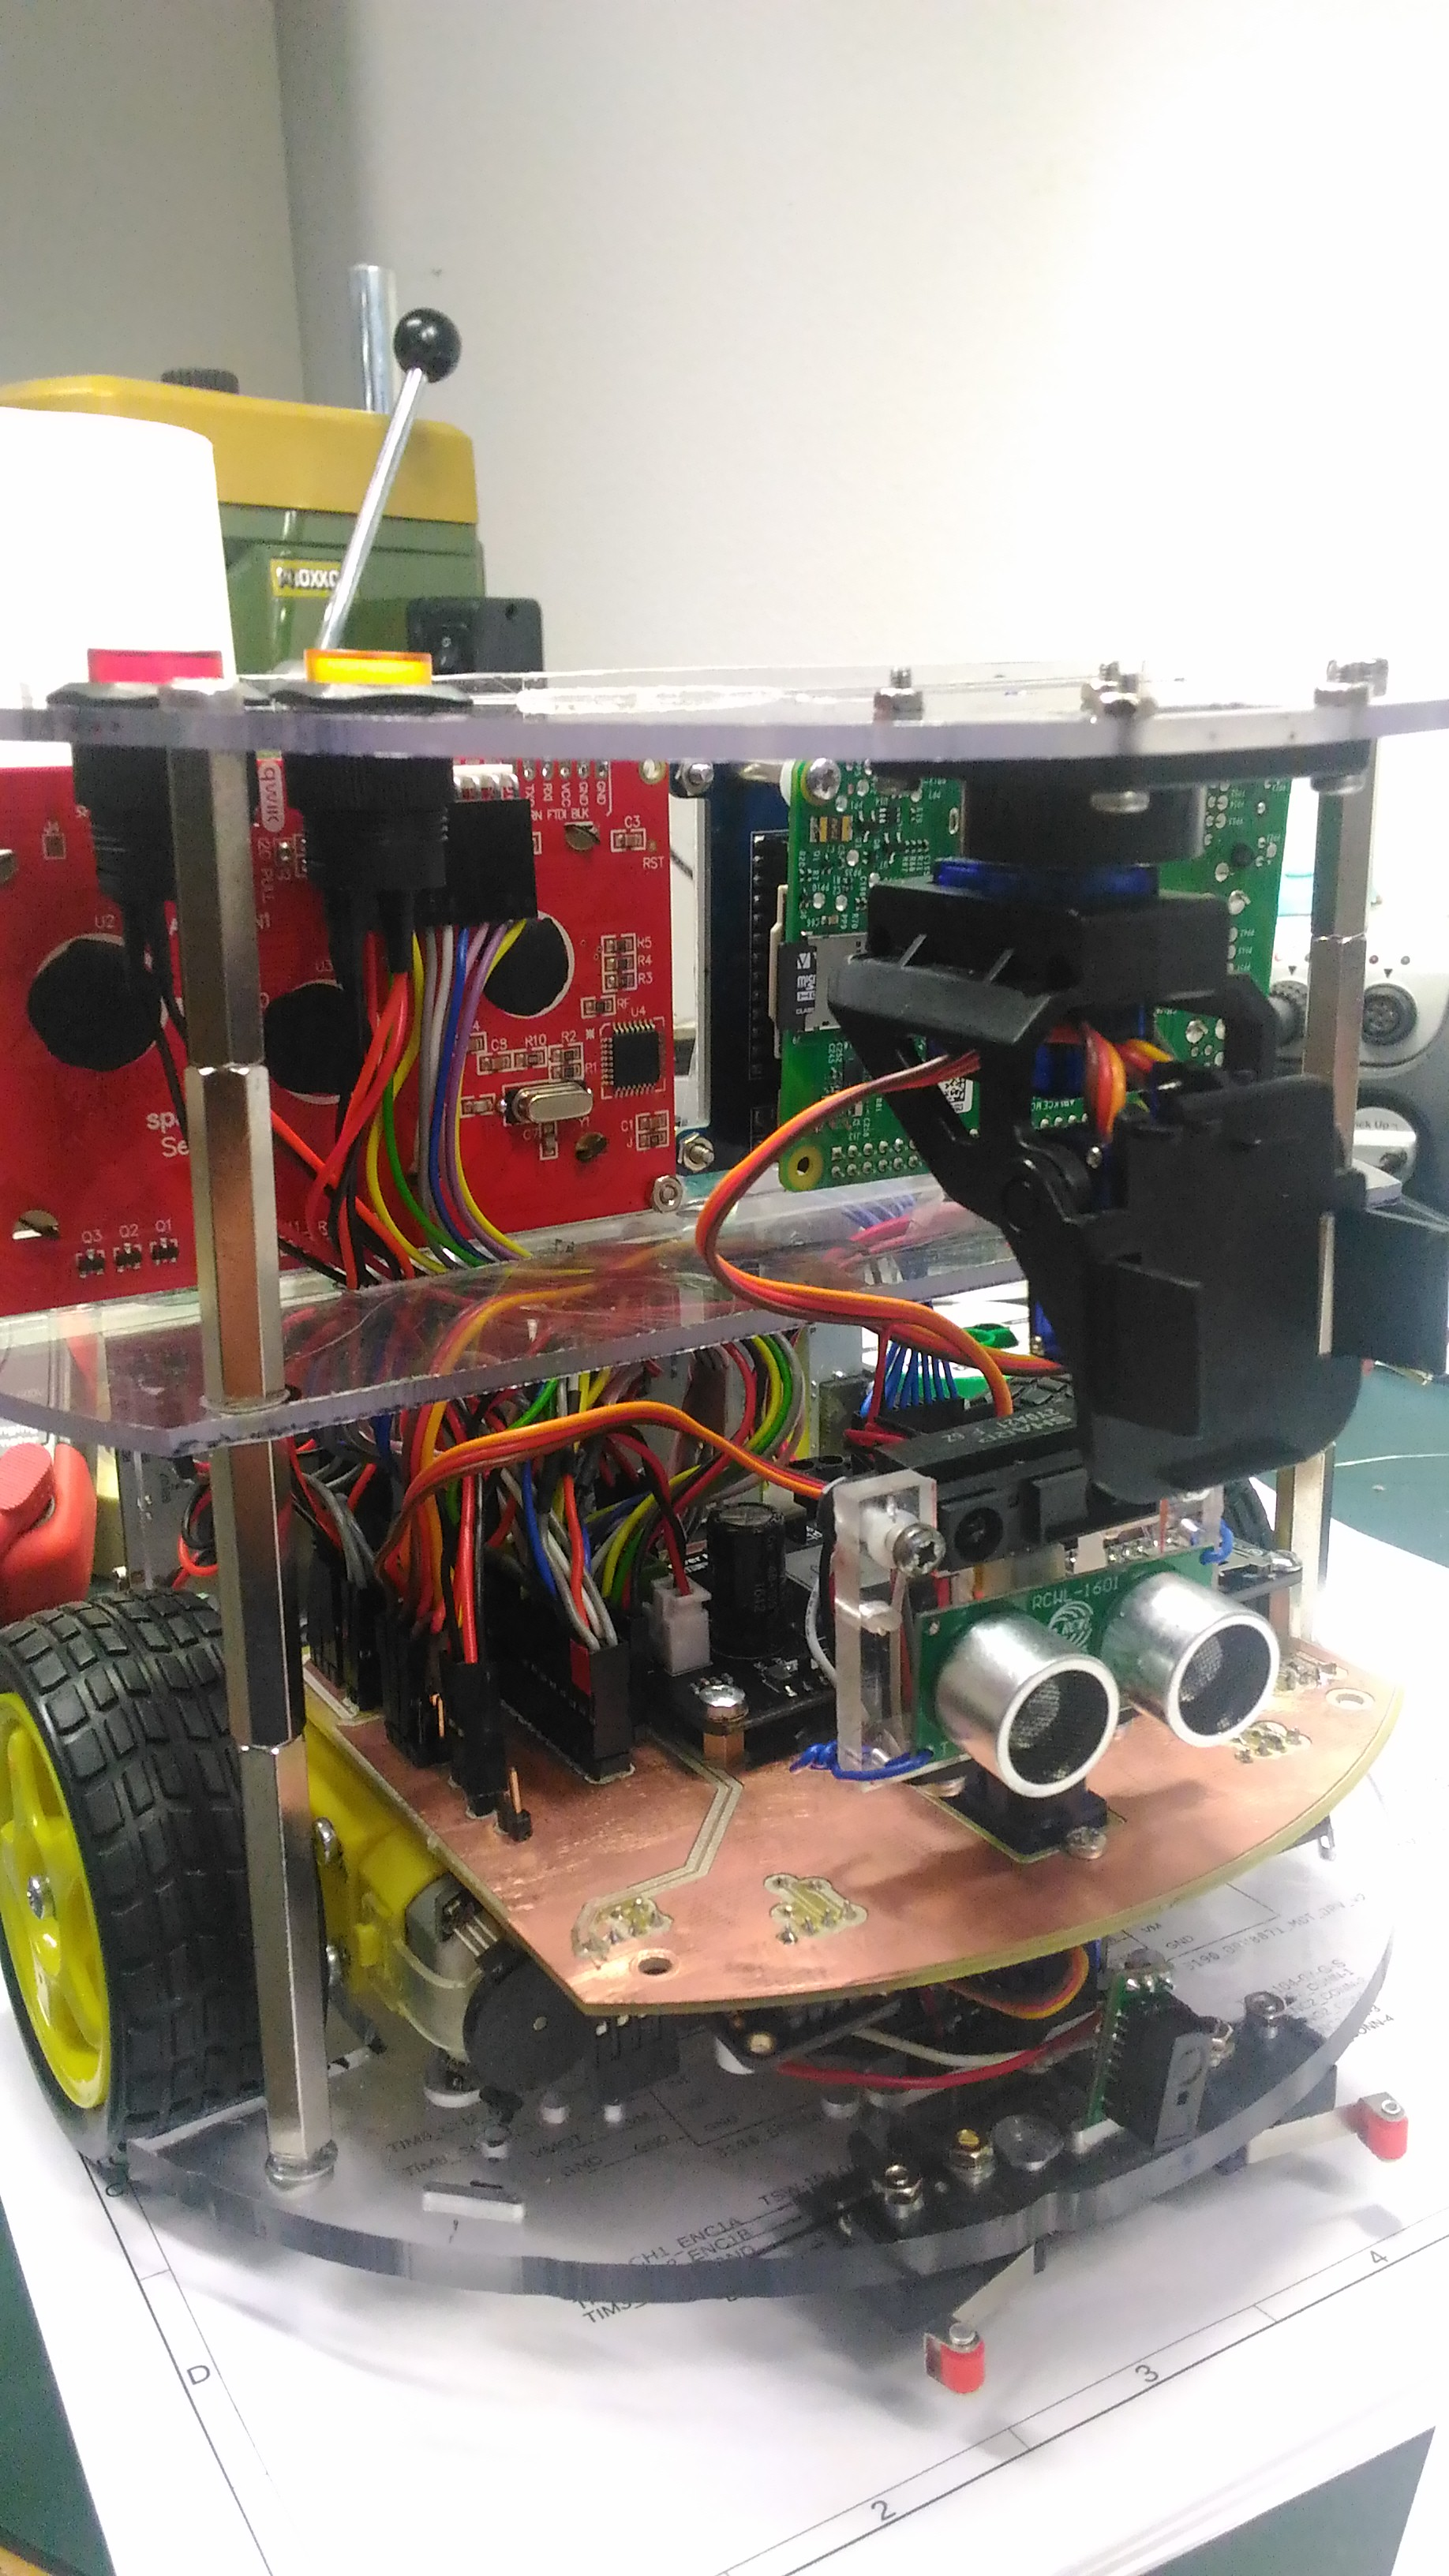
\includegraphics[width=0.3\textwidth,height=0.5\textwidth]{figures/turtlebot_2.jpg}
% 		\label{fig:tbot2}}
% 	\caption{The TurtleBot}
% \end{figure}

% \subsection{Another subsection}

% Lorem ipsum dolor sit amet, consectetur adipisci elit, sed eiusmod tempor incidunt ut labore et dolore magna aliqua. Ut enim ad minim veniam, quis nostrum exercitationem ullam corporis suscipit laboriosam, nisi ut aliquid ex ea commodi consequatur.

% \subsection{Another subsection}

% \begin{lstlisting}[language=C, caption={C code using listings}, label={lst:label} ]
% #include <stdio.h>
% int main()
% {
% 	// print hello to the console
% 	printf("Hello, world!");
% 	return 0;
% }
% \end{lstlisting}

% See code~\ref{lst:label}.




\clearpage
\appendix

\section{Section in the Appendix}
\label{sec:app1}

\subsection{Subsection in the Appendix}
\label{subsec:app2}

Additional relevant information...


\begin{thebibliography}{1}
	
	\bibitem{sx1509}
	SX1507/SX1508/SX1509. 2025. \textit{Sparkfun} [online]. [accessed 2025-4-22]. Available at: https://cdn.sparkfun.com/datasheets/BreakoutBoards/sx1509.pdf
	
	\bibitem{line_sensor}
	Pololu line sensor. 2025. \textit{Pololu.com} [online]. [accessed 2025-4-22]. Available at: https://www.pololu.com/docs/pdf/0J12/QTR-8x.pdf

\end{thebibliography}
\end{document}